\documentclass{article}
\usepackage{graphicx}
\usepackage[margin=1.5cm]{geometry}
\usepackage{amsmath}

\begin{document}

\title{Worksheet: Unit 1, Gauss' Law}
\author{Prof. Jordan C. Hanson}

\maketitle

\section{Memory Bank}

$\vec{E} \cdot \vec{A} = q_{enc}/\epsilon_0$ ... Gauss' Law

\section{Gauss' Law Procedure}

\begin{enumerate}
\item Observe Fig. \ref{fig:spheres4}.  The procedure to obtain the electric field of the spherical charge distribution is outlined below.
\begin{figure}[ht]
\centering
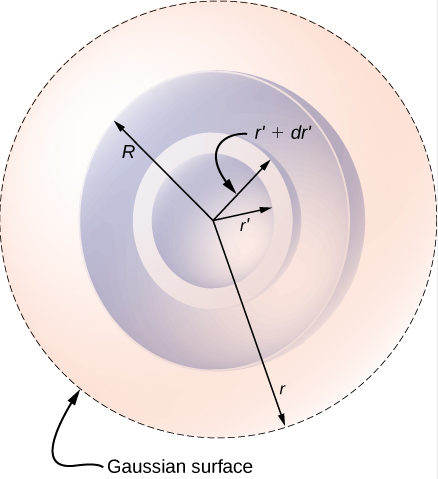
\includegraphics[width=0.25\textwidth]{spheres4.png}
\caption{\label{fig:spheres4} A charge distribution with spherical symmetry.}
\end{figure}
In Fig. \ref{fig:spheres4}, show that the volume of the spherical shell inside is $V_{shell} = 4\pi r'^2 dr'$.  Think about the volume of any spherical shell with thickness $dr'$. \\ \vspace{0.5cm}
\item Suppose the charge density is given by
\begin{equation}
\rho(r') = \rho_0 r'^n \label{eq:d}
\end{equation}
(a) What are the units of $\rho_0$? (b) What charge $dq$ is contained within $V_{shell}$, if the charge \textit{density} is given by Eq. \ref{eq:d}? \\ \vspace{1cm}
\item Write an integral from $0$ to some radius $r$ that sums up all the $dq$ inside of $r$. Make sure that it has the correct units.  \\ \vspace{1cm}
\item Perform the integral in the prior problem, and simplify.  What are the units of the answer?  (They should be Coulombs). \\ \vspace{1cm}
\item The result of the integral is the total charge contained within our sphere of radius $r$.  Insert this charge as the \textit{enclosed charge} in Gauss' law to obtain the E-field.  What do you put for $A$?
\end{enumerate}

\end{document}
